\documentclass{article}
\usepackage[margin=1in]{geometry}
\usepackage{natbib}
\usepackage{amsmath}
\usepackage{graphicx}
\usepackage{color}
\usepackage[procnames]{listings}
\usepackage{textcomp}
\usepackage{setspace}
\usepackage{palatino}

\usepackage{enumitem}
\setlist{nolistsep}

\usepackage{floatrow}
\usepackage{sidecap}
\sidecaptionvpos{figure}{c}
\usepackage{wrapfig}
\usepackage{float}
\usepackage{framed}
\usepackage{caption}

\definecolor{gray}{gray}{0.2}
\definecolor{green}{rgb}{0,0.5,0}
\definecolor{lightgreen}{rgb}{0,0.7,0}
\definecolor{purple}{rgb}{0.75,0,0.8}
\definecolor{darkred}{rgb}{0.6,0,0}
\definecolor{orange}{rgb}{1,0.3,0}
\definecolor{medblue}{rgb}{0, 0.5, 1}
\definecolor{lightgray}{rgb}{0.98, 0.98, 0.98}
\definecolor{medgray}{rgb}{0.93, 0.93, 0.93}
\definecolor{pink}{rgb}{0.8, 0, 0.8}


\setlength\parindent{0pt}
\usepackage[T1]{fontenc} % quotes

	
\newcommand{\code}[1]{\textbf{\texttt{\small{#1}}}}



\usepackage{hyperref}
\hypersetup{
	colorlinks=true, %set true if you want colored links
	linktoc=all,     %set to all if you want both sections and subsections linked
	linkcolor=blue,  %choose some color if you want links to stand out
	urlcolor=blue
}



\lstset{
		language=python,
		rulecolor=\color{black},
		frame=leftline,
		backgroundcolor=\color{medgray},
		numbers=left,
		numberstyle=\scriptsize,
		basicstyle=\ttfamily\footnotesize\setstretch{1.2},
		stringstyle=\color{red},
		showstringspaces=false,
		alsoletter={1234567890},
		otherkeywords={\ , \}, \{},
		breaklines=true,
		float,
		keywordstyle=\ttfamily,
		emph={access,and,as,break,class,continue,def,del,elif,else,%
			except,exec,finally,for,from,global,if,import,in,is,%
			lambda,not,or,pass,print,raise,return,try,while,assert},
		emphstyle=\color{medblue}\bfseries,
		emph={[2]self},
		emphstyle=[2]\color{gray},	
		emph={[4]ArithmeticError,AssertionError,AttributeError,BaseException,%
			DeprecationWarning,EOFError,Ellipsis,EnvironmentError,Exception,%
			False,FloatingPointError,FutureWarning,GeneratorExit,IOError,%
			ImportError,ImportWarning,IndentationError,IndexError,KeyError,%
			KeyboardInterrupt,LookupError,MemoryError,NameError,None,%
			NotImplemented,NotImplementedError,OSError,OverflowError,%
			PendingDeprecationWarning,ReferenceError,RuntimeError,RuntimeWarning,%
			StandardError,StopIteration,SyntaxError,SyntaxWarning,SystemError,%
			SystemExit,TabError,True,TypeError,UnboundLocalError,UnicodeDecodeError,%
			UnicodeEncodeError,UnicodeError,UnicodeTranslateError,UnicodeWarning,%
			UserWarning,ValueError,Warning,ZeroDivisionError,abs,all,any,apply,%
			basestring,bool,buffer,callable,chr,classmethod,cmp,coerce,compile,%
			complex,copyright,credits,delattr,dict,dir,divmod,enumerate,eval,%
			execfile,exit,filter,float,frozenset,getattr,globals,hasattr,%
			hash,help,hex,id,input,int,intern,isinstance,issubclass,iter,len,%
			license,list,locals,long,map,max,min,object,oct,open,ord,pow,property,%
			quit,range,raw_input,reduce,reload,repr,reversed,round,set,setattr,%
			slice,sorted,staticmethod,str,sum,super,tuple,unichr,unicode,%
			vars,xrange,zip},
		emphstyle=[4]\color{blue}\bfseries,
		emph={[5]construct_model,assign_name,num_classes,codon_model,read_tree,print_tree,%
			branch_het,site_het,construct_frequencies,Site,Evolver,Genetics,%
			MatrixBuilder,aminoAcid_Matrix,nucleotide_Matrix,mechCodon_Matrix,%
			mutSel_Matrix,ECM_Matrix,EvoModels,Model,CodonModel,Tree,Partition,%
			StateFrequencies,EqualFrequencies,RandomFrequencies,CustomFrequencies,%
			ReadFrequencies,EmpiricalModelFrequencies},
		emphstyle=[5]\color{purple}\bfseries,		
		upquote=true,
		morecomment=[s][\color{darkred}]{"""}{"""},
		morecomment=[s][\color{darkred}]{'''}{'''},
		commentstyle=\color{green}\slshape,
		literate={>>>}{\textbf{\textcolor{orange}{>{>}>}}}3%
		{...}{{\textcolor{gray}{...}}}3,
		procnamekeys={def,class},
		procnamestyle=\color{green}\textbf,
		tabsize=4	
}


% Python for external files
\newcommand\pythonexternal[2][]{{
		\lstinputlisting[#1]{#2}}}

% Python for inline
\newcommand\pythoninline[1]{{\lstinline!#1!}}



\begin{document}


\title{User manual for Pyvolve v1.0}
\author{Stephanie J. Spielman}
\date{}
\maketitle

\tableofcontents

\section{Introduction}

Pyvolve (pronouced ``pie-volve'') is an open-source python module for simulating genetic data along a phylogeny according to Markov models of sequence evolution, according to standard methods \cite{Yang2006}. The module is available for download on \href{https://github.com/sjspielman/pyvolve/releases}{github} (and see \href{http://sjspielman.org/pyvolve/}{here} for API documentation). Note that Pyvolve has several dependencies, including \href{http://biopython.org/wiki/Download}{BioPython}, \href{http://www.scipy.org/install.html}{NumPy}, and \href{http://www.scipy.org/install.html}{SciPy}. These modules must be properly installed and in your python path for Pyvolve to work properly. Please file any and all bug reports on the github repository \href{https://github.com/sjspielman/pyvolve/issues}{Issues} section.

Pyvolve is written such that it can be seamlessly integrated into your python pipelines without having to interface with external software platforms. However, please note that for extremely large (e.g. $>$1000 taxa) and/or extremely heterogenous simulations (e.g. where each site evolves according to a unique evolutionary model), Pyvolve may be quite slow and thus may take several minutes to run. Faster sequence simulators you may find useful include (but are certainly not limited to!) \href{http://abacus.gene.ucl.ac.uk/software/indelible/}{Indelible} \cite{Fletcher2009} and  \href{http://bioinfolab.unl.edu/~cstrope/iSG/}{indel-Seq-Gen} \cite{Strope2007}. 

Pyvolve supports a variety of evolutionary models, including the following:
\begin{itemize}
	\item Nucleotide Models 
	\begin{itemize}
		\item Generalized time-reversible model \cite{GTR} and all nested variants
	\end{itemize}
	\item Amino-acid exchangeability models 
	\begin{itemize}
		\item JTT \cite{JTT}, WAG \cite{WAG}, and LG \cite{LG}
	\end{itemize}
	\item Codon models
	\begin{itemize}
		\item Mechanistic ($dN/dS$) models (MG-style \cite{MG94} and GY-style \cite{GY94})
		\item Empirical codon model \cite{ECM}
	\end{itemize}
	\item Mutation-selection models
	\begin{itemize}
		\item Halpern-Bruno model \cite{HB98}, implemented for codons and nucleotides
	\end{itemize}
\end{itemize}
Note that it is also possible to specify custom matrices (detailed in section~\ref{sec:custom} below). Both site- and branch- (temporal) heterogeneity are supported. A detailed and highly-recommended overview of Markov process evolutionary models, for DNA, protein, and codons, is available in the book \emph{Computational Molecular Evolution}, by Ziheng Yang \citep{Yang2006}.

%\section{Special features in pyvolve}
%pyvolve includes several novel options not available (to my knowledge) in other sequence simulation softwares.
%\subsection{Custom rate-matrix specification}
%pyvolve comes with many standard evolutionary models, but it also allows you to specify your own custom rate matrix.
%\subsection{"Noisy" branch lengths}
%Rather than only applying a given branch length, as it appears in the specified phylogeny, to all sites as they evolve along that branch, pyvolve provides the option to include noise in these branch lengths. For example, if a branch length is equal to 0.1, then sites along that branch can evolve with normally-distributed branch lengths that have a mean of 0.1.
%\subsection{Neutral matrix scaling}. 
%By convention, matrices are scaled such that the mean substitution rate is 1. However, this can cause some confounding issues when multiple matrices control the evolutionary process, particularly in cases of codon model heterogeneity. The standard scaling approach would specify that a site evolving with $dN/dS = 2$ experiences the same average number of substitution as would a site evolving with $dN/dS = 0.05$. Biologically, this outcome is rather implausible. Therefore, we provide a novel scaling approach, "neutral", which scales the matrix such that the mean \textit{neutral} substitution rate is 1. In the context of codon models, this means that the mean number of substitutions increases linearly with increasing $dN/dS$.


\setlength{\parskip}{12pt}
\section{Basic Usage}

Similar to other simulation platforms, Pyvolve evolves sequences in groups of \textbf{partitions}. Each partition has an associated size and model (or set of models, if branch heterogeneity is desired). All partitions will evolve according to the same phylogeny; if you wish to have each partition evolve according to a distinct phylogeny, I recommend performing several simulations and then merging the resulting alignments in the post-processing stage. 

The general framework for a simple simulation is given below. In order to simulate sequences, you must define the phylogeny along which sequences evolve as well as any evolutionary model(s) you'd like to use. Each evolutionary model has associated parameters which you can customize, as detailed in Section~\ref{sec:evomodels}.

\begin{lstlisting}
######### General pyvolve framework #########
#############################################

# Import the Pyvolve module
import pyvolve

# Read in phylogeny along which Pyvolve should simulate
my_tree = pyvolve.read_tree(file = "file_with_tree_for_simulating.tre")

# Define and construct evolutionary models
my_model = pyvolve.Model(<model_type>, <custom_model_parameters>)
my_model.construct_model()

# Define partitions
my_partition = pyvolve.Partition(models = my_model, size = 100)

# Evolve partitions with the callable Evolver() class
my_evolver = pyvolve.Evolver(tree = my_tree, partitions = my_partition)
my_evolver() # evolve sequences
\end{lstlisting}

\code{Evolver()} will produce several output files, including the simulated data, as detailed in Section~\ref{sec:output_files}.

$<$model\_type$>$ is the type of model matrix. $<$custom\_model\_parameters$>$ is a \textit{dictionary} of parameters for your chosen model. See below for available model types and associated parameter keys.



\section{Defining phylogenies}\label{sec:phylogeny}

Phylogenies may be specified either as a newick tree string or by providing the name of a file that contains the newick tree. To provide a phylogeny, use the \code{read\_tree} function.
\begin{lstlisting}
# Read phylogeny from file with the argument "file"
phylogeny = read_tree(file = "/path/to/tree/file.tre")

# Read phylogeny from string with the argument "tree"
phylogeny = read_tree(tree = "(t4:0.785,(t3:0.380,(t2:0.806,(t5:0.612,t1:0.660):0.762):0.921):0.207);")
\end{lstlisting}

To implement branch (temporal) heterogeneity, in which different branches on the phylogeny evolve according to different models, you will need to specify \emph{model flags} at particular nodes in the newick tree, as detailed in Section~\ref{sec:branchhet}.

Further, to assess that a phylogeny has been parsed properly (or to determine the automatically-assigned names of internal nodes), use the \code{print\_tree} function:
\begin{lstlisting}
# Read phylogeny from string
phylogeny = read_tree(tree = "(t4:0.785,(t3:0.380,(t2:0.806,(t5:0.612,t1:0.660):0.762):0.921):0.207);")

# Print the parsed phylogeny
print_tree(phylogeny)
## Output from the above statement:
'''
 root None None
     t4 0.785 None
     internal_node3 0.207 None
         t3 0.38 None
         internal_node2 0.921 None
              t2 0.806 None
              internal_node1 0.762 None
                  t5 0.612 None
                  t1 0.66 None
'''
\end{lstlisting}
In the above output, tabs represent nested hierarchies in the phylogeny. Each line shows the node name (either a tip name, "root", or an internal node), the branch length leading to that node, and the model flag associated with that node. This final value will be \code{None} if model flags (as detailed in Section~\ref{sec:branchhet})are not provided in the phylogeny.



\section{Defining Evolutionary Models}\label{sec:evomodels}

The evolutionary models built into Pyvolve are outlined in the Introduction. All models used in simulation must be defined using the \code{Model()} class, the basic usage of which is detailed here.

\subsection{Nucleotide Models}\label{sec:nucleotide_basic}

Nucleotide rate matrix elements, for the substitution from nucleotide $i$ to $j$, are generally given by 
\begin{equation}
q_{ij} = \mu_{ij} \pi_j
\end{equation}
where $\mu_{ij}$ describes the rate of change from nucleotide $i$ to $j$, and $\pi_j$ represents the equilibrium frequency of the target nucleotide $j$. Note that mutation rates are symmetric, e.g.\ $\mu_{ij} = \mu_{ji}$. 

By default, nucleotide models have equal mutation rates and equal equilibrium frequencies (corresponding to the Jukes-Cantor model \citep{JC69}). A basic model can be constructed with, 
\begin{lstlisting}
# Simple nucleotide model 
nuc_model = pyvolve.Model("nucleotide")
nuc_model.construct_model()
\end{lstlisting}

To customize a nucleotide model, include a custom-parameters dictionary as a second argument to \code{Model()} with optional keys \code{"mu"} for custom mutation rates and \code{"state\_freqs"} for custom equilibrium frequencies (see Section~\ref{sec:freqs} for details on frequency customization). 
\begin{lstlisting}
# Define mutation rates in a dictionary with keys giving the nucleotide pair
# Below, the rate from A to C is 0.5, and similarly C to A is 0.5
custom_mu = {'AC':0.5, 'AG':0.25, 'AT':1.23, 'CG':0.55, 'CT':1.22, 'GT':0.47} 

# Define custom frequencies, in order A C G T. This can be a list or numpy array.
freqs = [0.1, 0.45, 0.3, 0.15]

# Construct nucleotide model with custom mutation rates and frequencies.
nuc_model = pyvolve.Model( "nucleotide", {'mu':custom_mu, 'state_freqs':freqs} )
nuc_model.construct_model()
\end{lstlisting}
Note that any undefined mutation rates will be set to 1. Further, mutation rates are symmetric; if you provide a rate for $A \rightarrow T$, it will automatically be applied as the rate $T \rightarrow A$. 

As an alternate to \code{"mu"}, you can provide the key \code{"kappa"}, which corresponds to the transition:transversion ratio (e.g.\ for an HKY85  model \citep{HKY85}), in the custom-parameters dictionary. When kappa is specified, tranversion rates are set to 1, and transition rates are set to the provided value.

\begin{lstlisting}
# Construct nucleotide model with transition-to-transversion bias, and default frequencies
nuc_model = pyvolve.Model( "nucleotide", {"kappa":2.75, "state_freqs":freqs} )
nuc_model.construct_model()
\end{lstlisting}


\subsection{Amino-acid models}\label{sec:amino_basic}

Amino-acid exchangeability matrix elements, for the substitution from amino acod $i$ to $j$, are given by 
\begin{equation}
q_{ij} = r_{ij} \pi_j
\end{equation}
where $r_{ij}$ is a symmetric matrix which describes the probability of changing from amino acid $i$ to $j$, and $\pi_j$ is the equilibrium frequency of the target amino acid $j$. The $r_{ij}$ matrix corresponds to an empirically determined model, such as WAG \citep{WAG} or LG \citep{LG}. 

By default, Pyvolve assigns equal equilibrium frequencies. A basic amino-acid model can be constructed with, 
\begin{lstlisting}
# Simple amino-acid model 
aa_model = pyvolve.Model("WAG") # Here, WAG can be one of JTT, WAG, LG (case-insensitive)
aa_model.construct_model()
\end{lstlisting}

To customize an amino-acid model, specify the custom-parameters dictionary with the key \code{"state\_freqs"} for custom equilibrium frequencies (see Section~\ref{sec:freqs} for details on frequency customization). Note that amino-acid frequencies must be in the order A, C, D, E, ... Y. Further, to specify the \textit{model's} default equilibrium frequencies, use the pyvolve EmpiricalModelFrequencies class:
\begin{lstlisting}
# Define default WAG state frequencies
f = pyvolve.EmpiricalModelFrequencies("WAG") # model name is case-insensitive
freqs = f.construct_frequencies()

# Construct amino-acid model with WAG frequencies
aa_model = pyvolve.Model( "WAG", {"state_freqs":freqs} )
aa_model.construct_model()
\end{lstlisting}



\subsection{Mechanistic ($dN/dS$) codon models}\label{sec:mechcodon_basic}

GY-style \citep{GY94} matrix elements, for the substitution from codon $i$ to $j$, are generally given by 
\begin{equation}\label{eq:GY94}
q_{ij} = \left\{ 
\begin{array}{rl}
\mu_{o_it_j} \pi_j \alpha      & \text{synonymous change} \\
\mu_{o_it_j} \pi_j \beta       & \text{nonsynonymous change} \\
0                    & \text{multiple nucleotide changes} \\             
\end{array} \right.,
\end{equation}
where $\mu_{o_it_j}$ is the mutation rate (e.g.\ for a change AAA to AAC, the corresponding mutation rate would be A $\rightarrow$ C), $\pi_j$ is the frequency of the target \emph{codon} $j$, $\alpha$ is the rate of synonymous change, and $\beta$ is the rate of nonsynonymous change. In this framework, $\beta / \alpha$ corresponds to $dN/dS$.


MG-style \citep{MG94} matrix elements, for the substitution from codon $i$ to $j$, are generally given by 
\begin{equation}\label{eq:MGstyle}
q_{ij} = \left\{ 
\begin{array}{rl}
\mu_{o_it_j}\pi_{t_j} \alpha         &\text{synonymous change} \\
\mu_{o_it_j}\pi_{t_j} \beta  &\text{nonsynonymous change} \\
0                             &\text{multiple nucleotide changes}       
\end{array} \right. ,
\end{equation}
where $\mu_{o_it_j}$ is the mutation rate, $\pi_{t_j}$ is the frequency of the target \emph{nucleotide} $t_j$ (e.g.\ for a change AAA to AAC, the target nucleotide would be C), $\alpha$ is the rate of synonymous change, and $\beta$ is the rate of nonsynonymous change. In this framework, $\beta / \alpha$ corresponds to $dN/dS$. Further, mutation rates are symmetric.

Codon models \emph{require} that you specify a $dN/dS$ rate ratio as a parameter in the \code{params} dictionary. There are several options for specifying this value:
\begin{itemize}
	\item Specify a single parameter, \code{"omega"}. This option sets the synonymous rate to 1.
	\item Specify a single parameter, \code{"beta"}. This option sets the synonymous rate to 1.
	\item Specify a two parameters, \code{"alpha"} and \code{"beta"}. This option sets the synonymous rate to $\alpha$ and the nonsynonymous rate to $\beta$. Further, mutation rates are symmetric.
\end{itemize}

By default, Pyvolve assigns equal mutation rates and equal equilibrium frequencies. Basic mechanistic codon models can be constructed with,
\begin{lstlisting}
# Simple GY-style model (specify as GY94)
gy_model = pyvolve.Model("GY94", {'omega': 0.5})
gy_model.construct_model()

# Simple MG-style model (specify as MG94)
mg_model = pyvolve.Model("MG94", {'alpha': 1.04, 'beta': 0.67})
mg_model.construct_model()

# Specifying "codon" results in a *GY-style* model
codon_model = pyvolve.Model("codon", {'beta': 1.25})
codon_model.construct_model()
\end{lstlisting}

To customize a mechanistic codon model, include the optional keys \code{"mu"} for custom mutation rates and \code{"state\_freqs"} for custom equilibrium frequencies (see Section~\ref{sec:freqs} for details on frequency customization) in the custom-parameters dictionary. Note that codon frequencies must ordered alphabetically (AAA, AAC, AAG, ..., TTG, TTT) \emph{without} stop codons.

\begin{lstlisting}
# Define mutation rates in a dictionary with keys giving the nucleotide pair
# Below, the rate from A to C is 0.5, and similarly C to A is 0.5
custom_mu = {'AC':0.5, 'AG':0.25, 'AT':1.23, 'CG':0.55, 'CT':1.22, 'GT':0.47} 

# Construct codon model with custom mutation rates
codon_model = pyvolve.Model( "codon", {'mu':custom_mu, 'omega':0.55} )
codon_model.construct_model()
\end{lstlisting}
Note that any undefined mutation rates will be set to 1. Further, mutation rates are symmetric; if you provide a rate for $A \rightarrow T$, it will automatically be applied as the rate $T \rightarrow A$. 

As an alternate to \code{"mu"}, you can provide the key \code{"kappa"}, which corresponds to the transition:transversion ratio (e.g.\ for an HKY85  model \citep{HKY85}), in the custom-parameters dictionary. When kappa is specified, tranversion rates are set to 1, and transition rates are set to the provided value.
\begin{lstlisting}
# Construct codon model with transition-to-transversion bias, and default frequencies
codon_model = pyvolve.Model( "codon", {"kappa":2.75, "alpha":0.89, "beta":0.95} )
codon_model.construct_model()
\end{lstlisting}




\subsection{Mutation-selection models}\label{sec:mutsel_basic}
Mutation-selection (MutSel) model \citep{HB98} matrix elements, for the substitution from codon (or nucleotide) $i$ to $j$, are generally given by 
\begin{equation}
q_{ij} = \left\{ 
\begin{array}{rl}
	\mu_{ij} \frac{S_{ij}}{1-1/S_{ij}} &\text{single nucleotide change} \\\\
	0                                  &\text{multiple nucleotide changes} \\             
\end{array} \right.,
\end{equation} where $\mu_{ij}$ is the mutation rate, and where $S_{ij}$ is the scaled selection coefficient. The scaled selection coefficient indicates the fitness difference between the target and source state, e.g. $fitness_j - fitness_i$. Mutation rates in MutSel models are \emph{not} constrained to be symmetric (e.g. $\mu_{ij}$ need not be equal to $\mu_{ji}$). 

MutSel models are implemented both for codons and nucleotides, and they may be specified either with equilibrium frequencies or with fitness values. Note that equilibrium frequencies must sum to 1, but fitness values are not constrained in any way. (The relationship between equilibrium frequencies and fitness values for MutSel models is detailed in refs.\ \citep{HB98,SpielmanWilke2015}). Pyvolve automatically determines whether you are evolving nucleotides or codons based on the provided vector of equilibrium frequencies or fitness values; a length of 4 indicates nucleotides, and a length of 61 indicates codons. Note that, if you are constructing a codon MutSel model based on \emph{fitness} values, you can alternatively specify a vector of 20 fitness values, indicating amino-acid fitnesses (in the order A,C, D, E, ... Y). These fitness values will be directly assigned to codons, such that all synonymous codons will have the same fitness.


Basic nucleotide MutSel models can be constructed with,
\begin{lstlisting}
# Simple nucleotide MutSel model constructed from frequencies, with default (equal) mutation rates
nuc_freqs = [0.1, 0.4, 0.3, 0.2]
mutsel_nuc_model_freqs = pyvolve.Model("MutSel", {'state_freqs': nuc_freqs})
mutsel_nuc_model_freqs.construct_model()

# Simple nucleotide MutSel model constructed from fitness values, with default (equal) mutation rates
nuc_fitness = [1.5, 0.88, -4.2, 1.3]
mutsel_nuc_model_fits = pyvolve.Model("MutSel", {'fitness': nuc_fitness})
mutsel_nuc_model_fits.construct_model()
\end{lstlisting}

Basic codon MutSel models can be constructed with,
\begin{lstlisting}
import numpy as np # imported for convenient example frequency/fitness generation

# Simple codon MutSel model constructed from frequencies, with default (equal) mutation rates
codon_freqs = np.repeat(1./61, 61) # constructs a vector of equal frequencies, as an example
mutsel_codon_model_freqs = pyvolve.Model("MutSel", {'freqs': codon_freqs})
mutsel_codon_model_freqs.construct_model()

# Simple codon MutSel model constructed from codon fitness values, with default (equal) mutation rates
codon_fitness = np.random.normal(size = 61) # constructs a vector of normally distributed codon fitness values, as an example
mutsel_codon_model_fits = pyvolve.Model("MutSel", {'freqs': codon_fitness})
mutsel_codon_model_fits.construct_model()

# Simple codon MutSel model constructed from *amino-acid* fitness values, with default (equal) mutation rates
aa_fitness = np.random.normal(size = 20) # constructs a vector of normally distributed amino-acid fitness values, as an example
mutsel_codon_model_fits2 = pyvolve.Model("MutSel", {'freqs': aa_fitness})
mutsel_codon_model_fits2.construct_model()

\end{lstlisting}

As usual, for both nucleotide and codon MutSel models, mutation rates can additionally be customized with the \code{"mu"} key in the \code{params} dictionary. Note that mutation rates in MutSel models do not need to be symmetric, but if you specify a rate for $A \rightarrow C$ and no rate for $C \rightarrow A$, then Pyvolve will assume symmetry and assign $C \rightarrow A$ the same rate as $A \rightarrow C$. Again, the parameter \code{"kappa"} may instead be specified in the custom-parameters dictionary.


\subsection{Empirical codon models}\label{sec:ecm_basic}
\textbf{DO I EVEN WANT TO RETAIN THIS?}
\begin{equation}\label{eq:ecmrest}
q_{ij} = \left\{ 
\begin{array}{rl}
s^\ast_{ij} \pi_j \kappa(i,j) \alpha      &\text{synonymous change} \\
s^\ast_{ij} \pi_j \kappa(i,j) \beta       &\text{nonsynonymous change} \\
\end{array} \right.,
\end{equation}
Further, rest and unrest. The $\kappa(i,j)$ parameter is defined in their paper...

\subsection{Specifying mutation rates}\label{sec:mu}

Nucleotide, mechanistic codon ($dN/dS$), and mutation-selection (MutSel) models all use nucleotide mutation rates as parameters. By default, mutation rates are equal for all nucleotide changes (e.g.\ the Jukes Cantor model \citep{JC69}). These default settings can be customized, in the custom model parameters dictionary, in one of two ways:
\begin{enumerate}
	\item Using the key \code{"mu"} to define custom rates for any/all nucleotide changes
	\item Using the key \code{"kappa"} to specify a transition-to-transversion bias ratio (e.g.\ the HKY85 mutation model. \citep{HKY85})
\end{enumerate}
The value associated with the \code{"mu"} key should itself be a dictionary of mutation rates, with keys "AC", "AG", "AT", etc, such that, for example, the key "AC" represents the mutation rate from A to C. Importantly, nucleotide and codon models use symmetric mutation rates; therefore, if a rate for "AC" is defined, the same value will automatically be applied to the change C to A. Thus, there are a total of 6 nucleotide mutation rates you can provide for a custom nucleotide and/or mechanistic codon model. Note that any rates not specified will be set to 1.

Alternatively, MutSel models do not constrain mutation rates to be symmetric, and thus, for instance, the "AC" rate may be different from the "CA" rate. Thus, there are a total of 12 nucleotide mutation rates you can provide for a custom MutSel model. Again, if a rate for "AC" but not "CA" is defined, then the "AC" rate will be automatically applied to "CA". Any unspecified nucleotide rate pairs will be set to 1. 
\begin{lstlisting}
# Example using customized mutation rates to construct a nucleotide model
custom_mutation_rates = {"AC":1.5, "AG":0.5, "AT":1.75, "CG":0.6, "CT":1.25, "GT":1.88}
my_model = pyvolve.Model("nucleotide", {"mu": custom_mutation_rates})
my_models.construct_model()
\end{lstlisting}

If, instead, the key \code{"kappa"} is specified, then the mutation rate for all transitions (e.g.\ purine to purine or pyrimidine to pyrimidine) will be set to the specified value, and the mutation rate for all transversions (e.g.\ purine to pyrimidine or vice versa) will be set to 1.
\begin{lstlisting}
# Example using customized kappa to construct a nucleotide model
my_model = pyvolve.Model("nucleotide", {"kappa": 3.5})
my_models.construct_model()
\end{lstlisting}


\section{Defining Partitions}\label{sec:partitions}

Partitions are defined using the \code{Partition()} class, with two required keyword arguments: \code{models}, the evolutionary model(s) associated with this partition, and \code{size}, the number of positions (sites) to evolve within this partition.
\begin{lstlisting}
# Define a default nucleotide model
my_model = pyvolve.Model("nucleotide")
my_models.construct_model()

# Define a partition which evolves according to this model of 100 sites
my_partition = pyvolve.Partition(models = my_model, size = 100)
\end{lstlisting}

In cases of branch homogeneity (all branches evolve according to the same model), each partition is associated with a single model, as shown above. When branch hetergeneity is desired, a list of models used should be provided to the \code{models} argument (as detailed in Section~\ref{sec:branchhet}).



\section{Evolving sequences}\label{sec:evolver}

The callable class \code{Evolver()} is Pyvolve's engine for all sequence simulation. Defining an \code{Evolver()} instance requires two keyword arguments: \code{partitions}, either the name of a single partition or a list of partitions to evolve, and \code{tree}, the phylogeny along which sequences are simulated.

Examples below show how to define an \code{Evolver()} instance and then evolve sequences. The code below assumes that all partition and tree variables provided as arguments to \code{Evolver()} have been previously defined using \code{Partition()} and \code{read\_tree}, respectively.
\begin{lstlisting}
# Define an Evolver instance to evolve a single partition
my_evolver = pyvolve.Evolver(partitions = my_partition, tree = my_tree)
my_evolver() # evolve sequences

# Define an Evolver instance to evolve several partitions
my_multpart_evolver = pyvolve.Evolver(partitions = [partition1, partition2, partition3], tree = my_tree)
my_multpart_evolver() # evolve sequences
\end{lstlisting}



\subsection{Evolver output files}\label{sec:output_files}

By default, \code{Evolver()} will output three files, to the working directory, when called:
\begin{enumerate}
	\item \textbf{simulated\_alignment.fasta}, a FASTA-formatted file containing simulated data
	\item \textbf{site\_rates.txt}, a tab-delimited file indicating to which partition and rate category each simulated site belongs (described in Section~\ref{sec:ratefile})
	\item \textbf{site\_rates\_info.txt}, a tab-delimited file indicating the rate factors and probabilities associated with each rate category (described in Section~\ref{sec:infofile})
\end{enumerate}


In the context of complete homogeneity, in which all sites and branches evolve according to a single model, the files "site\_rates.txt" and "site\_rates\_info.txt" will not contain much useful information. However, when sites evolve under either site-wise or branch heterogeneity, these files will provide useful information for any necessary post-processing.

To change the output file names for any of those files, provide the arguments \code{seqfile} ("simulated\_alignment.fasta"), \code{ratefile} ("site\_rates.txt"), and/or \code{infofile} ("site\_rates\_info.txt") when initializing an \code{Evolver} instance:
\begin{lstlisting}
# Provide custom file names when initializing the Evolver instance
my_evolver = pyvolve.Evolver(tree = my_tree, partitions = my_partition, ratefile = "custom_ratefile.txt", infofile = "custom_infofile.txt", seqfile = "custom_seqfile.fasta" )
my_evolver() #evolve
\end{lstlisting}

To suppress the creation of any of these files, define the argument(s) as either \code{None} or \code{False}:
\begin{lstlisting}
# Only output a sequence file (suppress the ratefile and infofile)
my_evolver = pyvolve.Evolver(tree = my_tree, partitions = my_partition, ratefile = None, infofile = None)
my_evolver() #evolve
\end{lstlisting}

The output sequence file's format can be changed with the argument \code{seqfmt} to \code{Evolver()}. Pyvolve uses Biopython to write sequence files, so consult the Biopython AlignIO module documentation (or this nice \href{http://biopython.org/wiki/AlignIO}{wiki}) for available formats.
\begin{lstlisting}
# Save the sequence file as seqs.phy, in phylip format 
my_evolver = pyvolve.Evolver(tree = my_tree, partitions = my_partition, seqfile = "seqs.phy", seqfmt = "phylip")
my_evolver() #evolve
\end{lstlisting}

By default, the output sequence file will contain only the tip sequences. To additionally output all ancestral (including root) sequences, provide the argument \code{write\_anc = True} to \code{Evolver()}. Ancestral sequences will be included with tip sequences in the output sequence file (not in a separate file!). When ancestral sequences are written, the root sequence is denoted with the name "root", and internal nodes are named "internal\_node1", "internal\_node2", etc. To see precisely to which node each internal node name corresponds, it is useful to print the parsed newick tree with the function \code{print\_tree}, as explained in Section~\ref{sec:phylogeny}.
\begin{lstlisting}
# Output ancestral sequences along with the tip sequences
my_evolver = pyvolve.Evolver(tree = my_tree, partitions = my_partition, write_anc = True)
my_evolver() #evolve
\end{lstlisting}


\subsubsection{Interpreting the "site\_rates.txt" output file}\label{sec:ratefile}
The output file "site\_rates.txt" has three columns of data:
\begin{itemize}
	\item \textbf{Site\_Index}
	\begin{itemize}
		\item Indicates a given position in the simulated data (indexed from 1)
	\end{itemize}
	\item \textbf{Partition\_Index}
	\begin{itemize}
		\item Indicates the partition associated with this site
	\end{itemize}
	\item \textbf{Rate\_Category}
	\begin{itemize}
		\item Indicates the rate category index associated with this site
	\end{itemize}
\end{itemize}


The values in "Partition\_Index" are ordered, starting from 1, based on the \code{partitions} argument list specified when setting up the \code{Evolver()} instance. Similarly, the values in "Rate\_Category" are ordered, starting from 1, based on the rate heterogeneity lists (see Section~\ref{sec:sitehet} for details) specified when setting up the \code{Model()}/\code{CodonModel()} objects used in the respective partition.


\subsubsection{Interpreting the "site\_rates\_info.txt" output file}\label{sec:infofile}
The output file "site\_rates\_info.txt" provides more detailed rate information for each partition. This file has give columns of data:
\begin{itemize}
	\item \textbf{Partition\_Index}
	\begin{itemize}
		\item Indicates the partition index (can be mapped back to the Partition\_Index column in "site\_rates.txt")
	\end{itemize}
	\item \textbf{Model\_Name}
	\begin{itemize}
		\item Indicates the model name (note that, if no name provided, this is None. Also, only relevant for branch het)
	\end{itemize}
	\item \textbf{Rate\_Category}
	\begin{itemize}
		\item Indicates the rate category index (can be mapped back to the Rate\_Category column in "site\_rates.txt")
	\end{itemize}
	\item \textbf{Rate\_Probability}
	\begin{itemize}
		\item Indicates the probability of a site being in the respective rate category
	\end{itemize}
	\item \textbf{Rate\_Factor}
	\begin{itemize}
		\item Indicates either the rate scaling factor (for nucleotide and amino-acid models), or $dN/dS$ value for this rate category for codon models
	\end{itemize}
\end{itemize}

%By default, sequences will be output to a fasta-formatted file called "simulated\_alignment.fasta". Two additional tab-delimited files, called "site\_rates.txt" and "site\_rates\_info.txt" are also output. These files provide useful information when heterogeneity (either site or branch) is implemented. The former file indicates to which partition and rate category (if no rate heterogeneity specified, these values will all be 1) each site belongs, and the latter file provides more specific information about each rate category, in particular its associated partition, probability, and value.

















\section{Implementing site-wise rate heterogeneity}\label{sec:sitehet}

This section details how to implement heterogeneity in site-wise rates \emph{within} a partition.


\subsection{Nucleotide and amino-acid models}

Rate heterogeneity is modeled for nucleotide and empirical amino-acid models discretely, using either a discrete gamma distribution or a user-specified rate distribution. Rate heterogeneity is incorporated in a model when \code{.model\_construct()} is called. 

\subsubsection{Gamma-distributed rate categories}

Gamma-distributed heterogeneity is specified with two (or three) arguments to the \code{.model\_construct()} method:
\begin{itemize}
	\item \code{alpha}, the shape parameter of the discrete gamma distribution from which rates are drawn (Note: following convention, $\alpha = \beta$ in these distributions \citep{Yang2006}).
	\item \code{num\_cateogories}, the number of rate categories to draw
	\item \code{rate\_probs}, an optional list of probabilities for each rate category. If unspecified, all rate categories are equally probable. This list should sum to 1!
\end{itemize}

Examples for specifying gamma-distributed rate heterogeneity are shown below.

\begin{lstlisting}
# Gamma-distributed heterogeneity for a nucleotide model. Gamma shape parameter is 0.5, and 6 categories are specified. All categories have an equal probability
nuc_model_het = pyvolve.Model("nucleotide")
nuc_model_het.construct_model(alpha = 0.5, num_categories = 6)

# Gamma-distributed heterogeneity for a nucleotide model. Gamma shape parameter is 0.5, and 6 categories are specified. Categories are assigned specified probabilities
nuc_model_het = pyvolve.Model("nucleotide")
nuc_model_het.construct_model(alpha = 0.5, num_categories = 6, rate_probs = [0.2, 0.3, 0.3, 0.1, 0.05, 0.05])

# Gamma-distributed heterogeneity for an amino-acid model. Gamma shape parameter is 0.5, and 6 categories are specified. All categories have an equal probability
aa_model_het = pyvolve.Model("WAG")
aa_model_het.construct_model(alpha = 0.5, num_categories = 6)
\end{lstlisting}

\subsubsection{Custom-distributed rate categories}

A user-determined heterogeneity distribution is specified with one (or two) arguments to the \code{.model\_construct()} method:
\begin{itemize}
	\item \code{rate\_factors}, a list of scaling factors for each category
	\item \code{rate\_probs}, an optional list of probabilities for each rate category. If unspecified, all rate categories are equally probable. This list should sum to 1!
\end{itemize}

Examples for specifying custom rate heterogeneity distributions are shown below.
\begin{lstlisting}
# Custom heterogeneity for a nucleotide model, with four equiprobable categories
nuc_model_het = pyvolve.Model("nucleotide")
nuc_model_het.construct_model(rate_factors = [0.4, 1.87, 3.4, 0.001])

# Custom heterogeneity for a nucleotide model, with four categories, each with a specified probability (i.e. rate 0.4 occurs with a probability of 0.15, etc.)
nuc_model_het = pyvolve.Model("nucleotide")
nuc_model_het.construct_model(rate_factors = [0.4, 1.87, 3.4, 0.001], rate_probs = [0.15, 0.25, 0.2, 0.5])

# Gamma-distributed heterogeneity for an amino-acid model, with four equiprobable categories
aa_model_het = pyvolve.Model("WAG")
aa_model_het.construct_model(rate_factors = [0.4, 1.87, 3.4, 0.001])
\end{lstlisting}



 
\subsection{Mechanistic codon models}

Due to the nature of mechanistic codon models, rate heterogeneity is not modeled with scalar factors, but with a distinct model for each rate (i.e.\, $dN/dS$ value) category. To setup heterogenous codon models, you must define models using the \code{CodonModel()}, rather than the \code{Model()} class. Defining such models is virtually the same as defining \code{(Model()} objects, except a \emph{list} of $dN/dS$ values should be provided to account for rate heterogeneity. As with standard codon models, you can provide $dN/dS$ values with keys \code{"omega"}, \code{"beta"}, or \code{"alpha"} and \code{"beta"} together (to incorporate both synonymous and nonsynonymous rate variation) in the custom model parameters dictionary.

By default, each discrete $dN/dS$ category will have the same probability. To specify custom probabilities, provide the argument \code{rate\_probs}, a list of probabilities, when calling the \code{.construct\_model()} method.

Examples for specifying heterogeneous mechanistic codon models are shown below (note that the GY94 model is shown in the examples, but as usual, both GY94 and MG94 are accepted.)
\begin{lstlisting}
# Define a heterogeneous codon model with dN/dS values of 0.1, 0.5, 1.0, and 2.5 . Categories are, by default, equally likely.
codon_model_het = pyvolve.CodonModel("GY94", {"omega": [0.1, 0.5, 1.0, 2.5]})
codon_model_het.construct_model()

# Define a heterogeneous codon model with dN/dS values of 0.102 (from 0.1/0.98) and 0.49 (from 0.5/1.02). Categories are, by default, equally likely.
codon_model_het = pyvolve.CodonModel("GY94", {"beta": [0.1, 0.5], "alpha": [0.98, 1.02]})
codon_model_het.construct_model()

# Define a heterogeneous codon model with dN/dS values of 0.102 (with a probability of 0.4) and 0.49 (with a probably of 0.6).
codon_model_het = pyvolve.CodonModel("GY94", {"beta": [0.1, 0.5], "alpha": [0.98, 1.02]})
codon_model_het.construct_model(rate_probs = [0.4, 0.6])
\end{lstlisting}


\subsection{Mutation-selection models}

Due to the nature of MutSel models, site-wise heterogeneity should be accomplished using a series of partitions, in which each partition evolves according to a unique MutSel model. These partitions can then be provided as a list when defining an \code{Evolver()} class.


\section{Implementing branch (temporal) heterogeneity}\label{sec:branchhet}

This section details how to implement branch (also known as temporal) heterogeneity within a partition, thus allowing different branches to evolve according to different models. To implement branch heterogeneity, your provided newick phylogeny should contain \emph{model flags} at particular nodes of interest. Model flags must be in the format \code{\_flagname\_} (i.e.\ with both a leading and a trailing underscore), and they should be placed after branch lengths or nodes (not after taxon names!). Note that model flags may be repeated throughout the tree, but the model associated with each model flag will always be the same. Once a model flag has been placed at a given node, all of that node's children will inherit that model. If a new model is specified in a child node, however, then this model will be applied downstream.

\begin{figure}[htpb]%{R}{0.7\textwidth}
	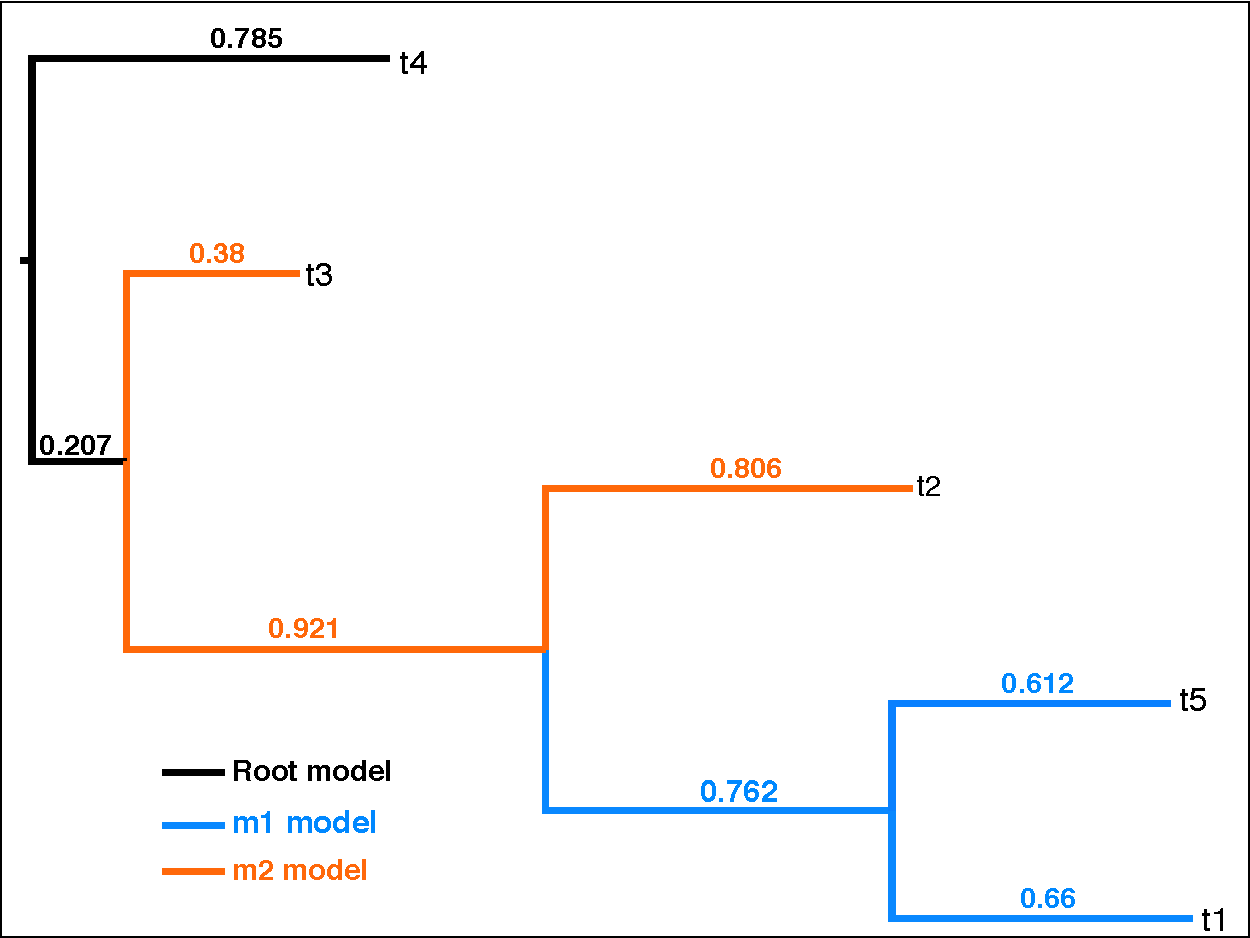
\includegraphics[width=3.75in]{treeflags.pdf}
	\caption{\label{fig:treeflags} The newick tree with model flags given by \\ \texttt{\scriptsize{"(t4:0.785,(t3:0.380,(t2:0.806,(t5:0.612,t1:0.660):0.762\_m1\_):0.921)\_m2\_:0.207);"}}
		indicates the model assignments shown.}
\end{figure}

For example, a tree specified as  \texttt{\scriptsize{(t4:0.785,(t3:0.380,(t2:0.806,(t5:0.612,t1:0.660):0.762\_m1\_):0.921)\_m2\_:0.207);}} will be interpreted as in Figure~\ref{fig:treeflags}. Trees with model flags, just like any other tree, are defined with the function \code{read\_tree}:
\begin{lstlisting}
# Define a tree with model flags m1 and m2, with a string
het_tree = pyvolve.read_tree( tree = "(t4:0.785,(t3:0.380,(t2:0.806,(t5:0.612,t1:0.660):0.762\_m1\_):0.921)\_m2\_:0.207);" )

# Define a tree with model flags m1 and m2, as read from a file
het_tree = pyvolve.read_tree( file = "/path/to/file/containing/tree/with/flags.tre" )
'''
\end{lstlisting}


All model flags specified in the newick phylogeny must have corresponding models, named identically (but without the leading/trailing underscores). To link a model to a model flag, specify a given model's name using the argument \code{name} in the \code{.construct\_model()} method. The model at the root of the tree will not have a specific model flag, but nonetheless a model must be used at the root (obviously), and indeed at all other nodes which are not assigned a model flag (not that all branches on the tree which are not assigned a model flag will evolve according to the model used at the root). To specify a model at the root of the tree, simply create a model, with a name, and indicate this name when defining your partition.

Examples for defining models with names are shown below (for demonstrative purposes, nucleotide models with extreme state frequency differences are used here):
\begin{lstlisting}
# Define the m1 model, with frequencies skewed for AT-bias
m1_model = pyvolve.Model("nucleotide", {'state_freqs':[0.4, 0.1, 0.1, 0.4]})
m1_model.construct_model(name = "m1")

# Define the m2 model, with frequencies skewed for GC-bias
m2_model = pyvolve.Model("nucleotide", {'state_freqs':[0.1, 0.4, 0.4, 0.1]})
m2_model.construct_model(name = "m2")

# Define the root model, with default equal nucleotide frequecies
root_model = pyvolve.Model("nucleotide")
root_model.construct_model(name = "root")
\end{lstlisting}

Alternatively, you can assign/re-assign a model's name with the \code{.assign\_name()} method:
\begin{lstlisting}
# ()Re-)assign the name of the root model
root_model.assign_name("new_root_model_name")
\end{lstlisting}



Finally, when defining the partition that uses all of these models, provide models as a list to the \code{models} argument. In addition, you \emph{must} specify the name of the model you wish to use at the root of the tree with the keyword argument \code{root\_model\_name} (the argument can be either the \code{.name} attribute or a the name as a string).
\begin{lstlisting}
# Define partition with branch heterogeneity, with 50 nucleotide positions
temp_het_partition = pyvolve.Partition(models = [m1_model, m2_model, root_model], size = 50, root_model_name = root_model.name) 
\end{lstlisting}



\section{Implementing branch-site heterogeneity}

Simulating according to so-called "branch-site" models, in which there are both site-wise and branch heterogeneity, is accomplished using the same strategies shown for each individual aspect (branch, Section~\ref{sec:branchhet} and site, Section~\ref{sec:sitehet}). However, there is a critical caveat to these models: all models within a given partition \emph{must} have the same number of rate categories. Furthermore, the rate probabilities must be the same across models within a partition; if different values for \code{rate\_probs} are indicated, then the probabilities provided for the \emph{root model} will be applied to all subsequent branch models. (Note that this behavior is identical for other simulation platforms, like Indelible \citep{Fletcher2009}.)

%In other words, because models must be re-assigned for different branches, the same \emph{number} of rate categories must hold.


\textcolor{red}{\textbf{CHECK THAT THIS CODE WILL WORK!!!!!}}
The example below shows how to specify a branch-site heterogeneous nucleotide model with two models, root and model1 (note that this code assumes that the provided phylogeny contained the flag \code{'\_model1\_}), when the rate categories are \emph{not} equiprobable.
\begin{lstlisting}
# Shared rate probabilities. Must be explicitly specified for all models (not just the root model)!
shared_rate_probs = [0.25, 0.3, 0.45]

# Construct a nucleotide model with 3 rate categories
root = Model("nucleotide")
root.construct_model(name = "root", rate_probs = shared_rate_probs, rate_factors = [1.5, 1.0, 0.05])

# Construct a second nucleotide model with 3 rate categories
model1 = Model("nucleotide")
mddel1.construct_model(name = "model1", rate_probs = shared_rate_probs, rate_factors = [0.06, 2.5, 0.11])

# Construct a partition with these models, defining the root model nameas "root"
part = Partition(models = [root, model1], root_model_name = "root", size = 50)
\end{lstlisting}


\section{Building a vector of equilibrium frequencies}\label{sec:freqs}

By default, Pyvolve assumes equal equilibrium frequencies (e.g.\ $0.25$ for nucleotides, $0.05$, for amino-acids, $1/61$ for codons). These conditions are not, however, very realistic. You can/should specify custom equilibrium frequencies for your simulations. Pyvolve provides a convenient class, called StateFrequencies, to help you with this step, with several child classes:
\begin{itemize}
	\item EqualFrequencies (\textbf{default}) \\ Sets frequencies as equal 
	\item RandomFrequencies \\ Computes (semi-)random frequencies
	\item CustomFrequencies \\ Computes frequencies from a user-provided dictionary of frequencies
	\item ReadFrequencies \\ Computes frequencies from a sequence or alignment file.
	\item EmpiricalModelFrequencies \\ Sets frequencies to default values for a given \emph{empirical} model		
\end{itemize}


All of these classes should be used with the following setup (the below code uses EqualFrequencies as a representative example):
\begin{lstlisting}
# Define frequency object
f = pyvolve.EqualFrequencies("nucleotide") # or "amino_acid" or "codon", depending on your simulation
frequencies = f.construct_frequencies() # returns a vector of equilibrium frequencies
\end{lstlisting}

The constructed vector of frequencies (named "frequencies" in the example above) can then be provided to the custom model parameters dictionary with the key \code{"state\_freqs"}. In addition, to conveniently save this vector of frequencies to a file, use the argument \code{savefile = <name\_of\_file>} when calling \code{.construct\_frequencies()}:
\begin{lstlisting}
# Define frequency object
f = pyvolve.EqualFrequencies("nucleotide")
frequencies = f.construct_frequencies(savefile = "my_frequency_file.txt") # returns a vector of equilibrium frequencies and saves them to file
\end{lstlisting}


\subsection{EqualFrequencies module}
Pyvolve uses this module to construct the default equilibrium frequencies. Usage should be relatively straight-forward, according to the example above.

\subsection{RandomFrequencies module}
This module is used to compute "semi-random" equilibrium frequencies. The resulting frequency distributions are not entirely random, but rather are virtually flat distributions with some amount of noise.

\subsection{CustomFrequencies module}
With this module, you can provide a dictionary of frequencies, using the argument \code{freq\_dict}, from which a vector of frequencies is constructed. The keys for this dictionary are the nucleotides, amino-acids (single letter abbreviations!), or codons, and the values should be the frequencies. Any states not included in this dictionary will be assigned a 0 frequency, so be sure the values in this dictionary sum to 1.

In the example below, CustomFrequencies is used to create a vector of amino-acid frequencies in which aspartate and glutamate each have a frequency of 0.25, and tryptophan has a frequency of 0.5. All other amino acids will have a frequency of 0.
\begin{lstlisting}
# Define CustomFrequencies object
f = pyvolve.CustomFrequencies("amino_acid", freq_dict = {"D":0.25, "E":0.25, "W":0.5})
frequencies = f.construct_frequencies()
\end{lstlisting}



\subsection{ReadFrequencies module}
The ReadFrequencies module can be used to compute equilibrium frequencies from a file of sequences and/or multiple sequence alignment. Frequencies can be computed either using all data in the file, or, if the file contains an alignment, using specified alignment column(s).
Note that Pyvolve will ignore all ambiguous characters present in this sequence file.

When specifying a file, use the argument \code{file}, and to specify the file format (e.g. FASTA or PHYLIP), use the argument \code{format}. Pyvolve uses Biopython to read the sequence file, so consult the Biopython AlignIO module documentation (or this nice \href{http://biopython.org/wiki/AlignIO}{wiki}) for available formats. Pyvolve assumes a default file format of FASTA, so the \code{format} argument is not needed when the file is FASTA.

\begin{lstlisting}
# Build frequencies using *all* data in the provided file
f = pyvolve.CustomFrequencies("amino_acid", file = "a_file_of_sequences.fasta")
frequencies = f.construct_frequencies()
\end{lstlisting}

To read frequencies from a specific column in a multiple sequence alignment, use the argument \code{columns}, which should be a list (\emph{indexed from 1}) of integers giving the column(s) which should be considered in frequency calculations.
\begin{lstlisting}
# Build frequencies using columns 1 through 5, inclusive of the alignment
f = pyvolve.CustomFrequencies("amino_acid", file = "alignment_file.fasta", columns = range(1,6))
frequencies = f.construct_frequencies()

# Build frequencies using columns 1 through 5, inclusive of the alignment
f = pyvolve.CustomFrequencies("amino_acid", file = "alignment_file.fasta", columns = range(1,6))
frequencies = f.construct_frequencies()

\end{lstlisting}



\subsection{EmpiricalModelFrequencies module}
The EmpiricalModelFrequencies model will return the default vector of equilibrium frequencies for a given empirical model [amino-acid models JTT, WAG, and LG and the codon model ECM, restricted and unrestricted versions (see ref.\ \citep{ECM} for details)]. These default frequencies correspond to the frequencies originally published with each respective matrix. To obtain these frequencies, provide, as an argument to EmpiricalModelFrequencies, the name of the desired model.
\begin{lstlisting}
# Obtain frequencies for the WAG model
f = pyvolve.CustomFrequencies("WAG")
frequencies = f.construct_frequencies()

# For the ECM models, use the argument "ECMrest" for restricted, and "ECMunrest" for unrestricted
f = pyvolve.CustomFrequencies("ECMrest") # restricted ECM frequencies
frequencies = f.construct_frequencies()
\end{lstlisting}




\subsection{Restricting frequencies to certain states}

When using the classes EqualFrequencies and RandomFrequencies, it is possible to specify that only certain states be considered during calculations using the \code{restrict} argument when defining the respective object. This argument takes a list of states (nucleotides, amino-acids, or codons) which should have non-zero frequencies. All states not included in this list will have a frequency of zero. Thus, by specifying this argument, frequencies will be distributed among the provided states. 

The following example will return a vector of amino-acid frequencies evenly divided among the five specified amino-acids; therefore, each amino acid in the \code{restrict} list will have a frequency of 0.2.
\begin{lstlisting}
# Compute equal frequencies among 5 specified amino acids
f = pyvolve.EqualFrequencies("amino_acid", restrict = ["A", "G", "V", "E", "F"])
frequencies = f.construct_frequencies()
\end{lstlisting}

Note that specifying this argument will have no effect on the CustomFrequencies, ReadFrequencies, or EmpiricalModelFrequencies classes.






\subsection{Converting frequencies between alphabets}

When defining a StateFrequencies variable, you always have to define the alphabet (nucleotide, amino acid, or codon) in which frequency calculations should be performed. However, it is possible to have the \code{.construct\_frequencies()} method return frequencies in a different alphabet, using the argument \code{type}. This argument takes a string specifying the desired type of frequencies returned, either "nucleotide", "amino\_acid", or "codon".

This functionality is probably most useful when used with the ReadFrequencies class; for example, you might want to obtain amino-acid frequencies from multiple sequence alignment of codons:
\begin{lstlisting}
# Define frequency object
f = pyvolve.ReadFrequencies("codon", file = "my_codon_alignment.fasta")
frequencies = f.construct_frequencies(type = "amino_acid")
\end{lstlisting}

As another example, you might want to obtain amino-acid frequencies which correspond to equal codon frequencies of $1/61$ each:
\begin{lstlisting}
f = pyvolve.EqualFrequencies("codon")
frequencies = f.construct_frequencies(type = "amino_acid") # returns a vector of amino-acid frequencies that correspond to equal codon frequencies
\end{lstlisting}

Alternatively, you can also go the other way (amino acids to codons):
\begin{lstlisting}
f = pyvolve.EqualFrequencies("amino_acid")
frequencies = f.construct_frequencies(type = "codon")
\end{lstlisting}
When converting amino acid to codon frequencies, Pyvolve assumes that there is \emph{no codon bias}, and assigns each synonymous codon the same frequency. Pyvolve does, however, allow you to specify codon bias by providing the argument, \code{codon\_bias}, to the \code{.construct\_frequencies()} method. This argument should be a value $x \in (0, 1]$ (exclusive of 0, inclusive of 1). Pyvolve will, for each amino acid, randomly select a preferred codon and assign this preferred codon a frequency $x$ times the parent amino acid's frequency. All other codons are designated as non-preferred, and the remaining frequency amount is divided equally among them. In this way, the overall amino acid frequency is preserved, but it is partitioned different among its constituent codons. For example, if the specified bias is 0.05, and a given 4-fold degenerate amino acid's overall frequency is 0.1, then (randomly selected) preferred codon for this amino acid will have a frequency of 0.05, and the remaining three non-preferred codons will each have frequencies of 0.05/3.



\section{Special Features}\label{sec:special}

\subsection{Matrix scaling options}\label{sec:scaling}

By convention, rate matrices are scaled such that the mean substitution rate is 1:
\begin{equation}\label{eq:scaling}
- \sum_{i=1} \pi_iq_{ii} = 1
\end{equation}
 \citep{GY94,Yang1994}. Using this regime, branch lengths explicitly indicate the expected number of substitutions per unit (nucleotide, amino acid, or codon). By default, Pyvolve will scale rate matrices according to equation~\ref{eq:scaling}, as this approach remains conventional in the field. 
 
Unfortunately, this scaling approach can lead to some unexpected results for modeling frameworks which contain explicit parameters for natural selection (mechanistic codon and MutSel models). For example, when multiple mechanistic codon ($dN/dS$) models are used, thus allowing for variable $dN/dS$ values across sites, multiple rate matrices must be used -- one matrix per $dN/dS$ value. This scaling approach, then, would cause sites with $dN/dS = 0.05$ to experience the same average number of substitutions as sites with $dN/dS = 2.5$. From a biological perspective, this result is undesirable, as sites with low $dN/dS$ values should evolve more slowly than sites with high $dN/dS$ values.
 
To overcome this issue, Pyvolve provides an option to scale matrices such that the mean \textit{neutral} substitution rate is 1. For $dN/dS$ codon models, this approach scales the matrix such that the mean number of substitutions when $dN/dS = 1$ is 1. For mutation-selection models (both nucleotide and codon), this approach scales the matrix such that the mean substitution rate is 1 when all states (nucleotides/codons) have equal fitness. Note that invoking neutral-scaling option has no effect on nucleotide or amino-acid models!

To invoke the neutral scaling, provide a third argument "neutral" when initializing a model:
\begin{lstlisting}
# Construct a codon model with neutral-scaling
m = pyvolve.Model("GY94", {"omega":0.5}, "neutral") # Indicate neutral scaling with a third argument, "neutral"
m.construct_model()
\end{lstlisting}

While we believe that this neutral scaling approach leads to more realistic simulated data, we urge caution when using this scaling approach. Most phylogenetic inference softwares and modeling frameworks (including HyPhy \citep{HYPHY} and PAML \citep{PAML}), scale matrices according to equation~\ref{eq:scaling}, and thus inferences on data simulated with neutral scaling may be confounded due to conventions in third-party softwares.

%In the context of codon models, this means that the mean number of substitutions increases linearly with increasing $dN/dS$.

\subsection{Specifying custom rate matrices}\label{sec:custom}

Rather than using a built-in modeling framework, you can specify a custom rate matrix. Any provided matrix must be a square matrix with dimensions of $4\times4$, $20\times20$, or $61\times61$ (for nucleotide, amino-acid, or codon evolution, respectively). Further, all rows in this matrix must sum to 0. Pyvolve will perform limited sanity checks on your matrix to ensure that these conditions are met, but beyond this, Pyvolve takes your matrix at face-value. In particular, Pyvolve will not scale the matrix in any manner.

Note that you can still specify custom equilibrium frequencies, but these frequencies will not be applied to any matrix scaling - they will be used only for sampling the root sequence in simulation.

To specify a custom rate matrix, provide the argument \code{"custom"} as the first argument when defining a \code{Model()} object, and provide your matrix in the parameters dictionary using the key \code{matrix}. 
Any custom matrix specified should be either a 2D numpy array or a python list of lists. Pyvolve orders nucleotides in the order ACGT, amino-acids in the order ACDEFGHIKLMNPQRSTVWY, and codons in the order AAA, AAC, AAG, ... TTT (without stop codons!). Below is an example of specifying a custom nucleotide rate matrix:
\begin{lstlisting}
# Define the custom rate matrix (4x4 for nucleotide evolution)
custom_matrix= np.array([[-1.0, 0.33, 0.33, 0.33], 
                         [0.25, -1.0, 0.25, 0.50], 
                         [0.10, 0.80, -1.0, 0.10],
                         [0.33, 0.33, 0.33, -1.0]] )

# Construct a model using the custom rate-matrix
custom_model = pyvolve.Model("model", {"matrix":custom_matrx})
custom_model.construct_model()
\end{lstlisting}


\subsection{Incorporating noise into branch lengths}\label{sec:noisybl}

Conventional sequence simulation algorithms apply a given branch length uniformly across a given branch. For example, if a given branch has a length of 0.1, then every site along that branch will evolve with a branch length of exactly 0.1. However, phylogenetic inference methods compute branch lengths as an average value for all sites along that branch, and there is no reasonable justification to assume all sites should have an identical branch length.

Therefore, Pyvolve allows you to specify some amount of noise in the branch lengths using the argument \code{noisy\_branch\_lengths = True} when defining an \code{Evolver()} object:
\begin{lstlisting}
# Specify some amount of noise in branch lengths
evolver = Evolver(partitions = my_partitions, tree = my_tree, noisy_branch_lengths = True)
\end{lstlisting}
In this scheme, the \emph{average} branch length for each branch will be the value specified in the newick phylogeny, but each site will evolve according to a slightly different value. Specifically, Pyvolve will sample, for each branch, branch lengths from a uniform distribution with a mean value equal to the branch length specified in the newick tree, and upper and lower bounds of $\pm$ 10\% of this branch length. For example, the range of values drawn for a branch length of 0.25 will fall in 0.225 - 0.275 (calculated from $0.25 \pm (0.1\times0.25)$). By default, 10 values will be drawn from this distribution, and these branch lengths will be randomly assigned to sites along the branch. 


These parameters can be further customized. To sample a different number of branch lengths per branch (rather than 10), specify the additional argument \code{noisy\_branch\_lengths\_n} when defining an \code{Evolver} object. You can provide either a specific number to this argument, or the word "full" to indicate that each site should have a uniquely-sampled branch length (note that specifying "full" might be quite slow!)
\begin{lstlisting}
# Specify 15 branch length categories per branch
evolver = Evolver(partitions = my_partitions, tree = my_tree, noisy_branch_lengths = True, noisy_branch_lengths_n = 15)
 
# Specify that every site should have a unique branch length
evolver = Evolver(partitions = my_partitions, tree = my_tree, noisy_branch_lengths = True, noisy_branch_lengths_n = "full")
\end{lstlisting}


Further, you can customize the uniform distribution's bounds with the argument \\ \code{noisy\_branch\_lengths\_scale}. The default value for this scale is 0.1, as described above. The scale value is applied as a percentage of the mean. For example, for a given branch length of 0.6 with a scale of 0.5, sampled branch lengths will be in the range 0.3 - 0.9 (calculated from $0.6 \pm (0.5\times0.6$)).
\begin{lstlisting}
# Specify a wider range for branch length sampling
evolver = Evolver(partitions = my_partitions, tree = my_tree, noisy_branch_lengths = True, noisy_branch_lengths_scale = 0.75)

# Specify a very narrow range for branch length sampling
evolver = Evolver(partitions = my_partitions, tree = my_tree, noisy_branch_lengths = True, noisy_branch_lengths_scale = 0.01)
\end{lstlisting}

To customize both the number of branch length categories and the range, provide all arguments:
\begin{lstlisting}
# Specify noisy branch lengths with wider sampling range and more categories
evolver = Evolver(partitions = my_partitions, tree = my_tree, noisy_branch_lengths = True, noisy_branch_lengths_n = 15, noisy_branch_lengths_scale = 0.75)
\end{lstlisting}


Note that the arguments \code{noisy\_branch\_lengths\_n} and \code{noisy\_branch\_lengths\_scale} will be ignored if \code{noisy\_branch\_lengths} is not set to \code{True}.


%\section{Insertions and Deletions}
%
%At this time, Pyvolve does not support insertions and deletions ("indels"). The main reason for this is that there is currently no obvious way to specify the evolution of inserted sequences. Standard simulation approaches will evolve inserted sequences like any other region: the inserted sequence will be drawn from a specified equilibrium frequency distribution, and then the inserted region will evolve according to a specified rate matrix. Typically, these parameters are taken directly from the model used in the insertion region. This setup is not, however, ideal... 


%\noindent This is my first python example:
%\pythonexternal{script.py}












\bibliographystyle{plain}
\bibliography{citations}





\end{document}